
%%%%%%%%%%%%%%%%%%%%%%%%%%%%%%%%%%%%%%%%%%%%%%%%%%%%%%%%%%%%%%%%%%%%%%%%%%%%%%%%%%%%%%%
%%%%%%%%%%%%%%%%%%%%%%%%%%%%%%%%%%%%%%%%%%%%%%%%%%%%%%%%%%%%%%%%%%%%%%%%%%%%%%%%%%%%%%%
% 
% This top part of the document is called the 'preamble'.  Modify it with caution!
%
% The real document starts below where it says 'The main document starts here'.

\documentclass[12pt]{article}

\usepackage{amssymb,amsmath,amsthm}
\usepackage[top=1in, bottom=1in, left=1.25in, right=1.25in]{geometry}
\usepackage{fancyhdr}
\usepackage{enumerate}
\usepackage{listings}
\usepackage{graphicx}
\usepackage{float}

\usepackage{mwe}
\usepackage{caption}
\usepackage{subcaption}
% Comment the following line to use TeX's default font of Computer Modern.
\usepackage{times,txfonts}



\makeatletter
\renewcommand*\env@matrix[1][*\c@MaxMatrixCols c]{%
  \hskip -\arraycolsep
  \let\@ifnextchar\new@ifnextchar
  \array{#1}}
\makeatother

\newtheoremstyle{homework}% name of the style to be used
  {18pt}% measure of space to leave above the theorem. E.g.: 3pt
  {12pt}% measure of space to leave below the theorem. E.g.: 3pt
  {}% name of font to use in the body of the theorem
  {}% measure of space to indent
  {\bfseries}% name of head font
  {:}% punctuation between head and body
  {2ex}% space after theorem head; " " = normal interword space
  {}% Manually specify head
\theoremstyle{homework} 

% Set up an Exercise environment and a Solution label.
\newtheorem*{exercisecore}{Exercise \@currentlabel}
\newenvironment{exercise}[1]
{\def\@currentlabel{#1}\exercisecore}
{\endexercisecore}

\newcommand{\localhead}[1]{\par\smallskip\noindent\textbf{#1}\nobreak\\}%
\newcommand\solution{\localhead{Solution:}}

%%%%%%%%%%%%%%%%%%%%%%%%%%%%%%%%%%%%%%%%%%%%%%%%%%%%%%%%%%%%%%%%%%%%%%%%
%
% Stuff for getting the name/document date/title across the header
\makeatletter
\RequirePackage{fancyhdr}
\pagestyle{fancy}
\fancyfoot[C]{\ifnum \value{page} > 1\relax\thepage\fi}
\fancyhead[L]{\ifx\@doclabel\@empty\else\@doclabel\fi}
\fancyhead[C]{\ifx\@docdate\@empty\else\@docdate\fi}
\fancyhead[R]{\ifx\@docauthor\@empty\else\@docauthor\fi}
\headheight 15pt

\def\doclabel#1{\gdef\@doclabel{#1}}
\doclabel{Use {\tt\textbackslash doclabel\{MY LABEL\}}.}
\def\docdate#1{\gdef\@docdate{#1}}
\docdate{Use {\tt\textbackslash docdate\{MY DATE\}}.}
\def\docauthor#1{\gdef\@docauthor{#1}}
\docauthor{Use {\tt\textbackslash docauthor\{MY NAME\}}.}
\makeatother

% Shortcuts for blackboard bold number sets (reals, integers, etc.)
\newcommand{\Reals}{\ensuremath{\mathbb R}}
\newcommand{\Nats}{\ensuremath{\mathbb N}}
\newcommand{\Ints}{\ensuremath{\mathbb Z}}
\newcommand{\Rats}{\ensuremath{\mathbb Q}}
\newcommand{\Cplx}{\ensuremath{\mathbb C}}
%% Some equivalents that some people may prefer.
\let\RR\Reals
\let\NN\Nats
\let\II\Ints
\let\CC\Cplx
%%%%%%%%%%%%%%%%%%%%%%%%%%%%%%%%%%%%%%%%%%%%%%%%%%%%%%%%%%%%%%%%%%%%%%%%%%%%%%%%%%%%%%%
%%%%%%%%%%%%%%%%%%%%%%%%%%%%%%%%%%%%%%%%%%%%%%%%%%%%%%%%%%%%%%%%%%%%%%%%%%%%%%%%%%%%%%%
% 
% The main document start here.

% The following commands set up the material that appears in the header.




%  \textbf{Code:}
%  \begin{center}
%  \lstinputlisting[basicstyle = \footnotesize]{}
%  \end{center}
%  
%  \begin{footnotesize}
%  \begin{verbatim}
%    
%  \end{verbatim}
%  \end{footnotesize}
%  
%  
%  \begin{figure}[H]
%    \begin{center}
%      \caption{}
%    \includegraphics[width = \textwidth]{}
%    \end{center}
%  \end{figure}




\doclabel{Stat 461: Homework 8}
\docauthor{Stefano Fochesatto}
\docdate{\today}

\begin{document}
\begin{exercise}{1} The idea of credit scorning is that you try to classify people into a group that will pay the money back and a group that won't. We'll use a version of a well-known dataset called Kredit, 
  which contained data from 1000 germans. This version we'll use is from kaggle.\\
  \begin{enumerate}
    \item[a.] Load the csv german\_credit\_data.\\
    \solution Reading in the data we find that the checking and saving account variables contain all the missing values. Simply removing all the rows with missing values reduces our number of observations to 522, which is about half.
    I am not necessary sure we should be throwing out so much of our data, for two variables which are not entirely indicative of an individuals credit responsibility. There are a few actions we can take to try and save this data.
    We could impute the medium value for these missing values, use a discriminant method that is robust to missing values like decision trees, or we could simply drop these categorical predictors. I ended up deciding to remove the variables mainly because KNN performs better on lower dimensional data.
    Plotting the pair plots shows us that this data is not in the slightest separable so I don't think any method will perform very well at all; this is also corroborated by the manova analysis below.\\
      \textbf{Code:}
      \begin{center}
      \lstinputlisting[basicstyle = \footnotesize]{r1.txt}
      \end{center}
      \vspace{.15in}
      \begin{figure}[H]
        \begin{center}
          \caption{Pair Plot of Variables Colored by Kredit.}
        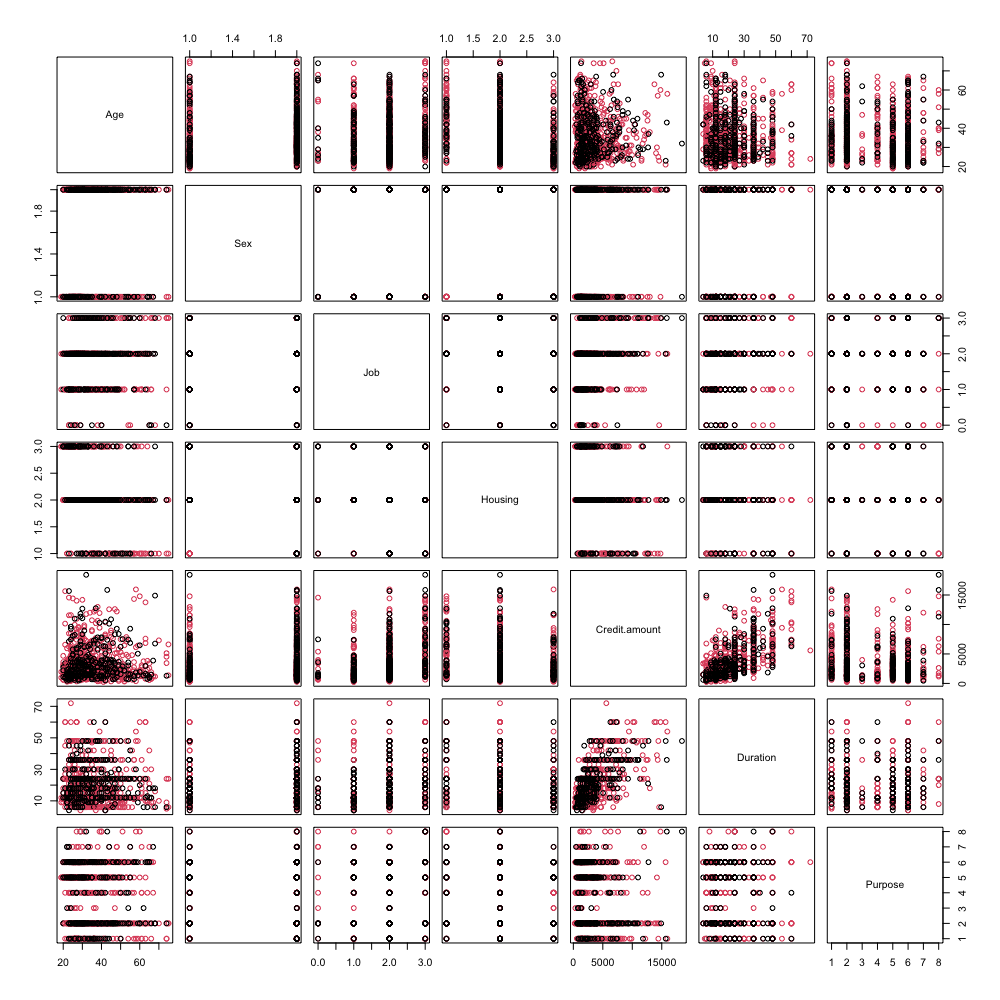
\includegraphics[width = \textwidth]{Rplot03.png}
        \end{center}
      \end{figure}


    \item[b.] Try a k-nearest neighbors classification. Select a value of k that you think is reasonable, then split the data into a training set and a testing set, then look at how well it classified the test data.\\
    \solution There are several ways to decide a value of $k$, I have seen that as a rule of thumb some people simply decide on the square root of the number of observations in the data. Since our data has 1000 observations
    we will try with $k = \sqrt(1000) \approx 32$. Ideally we would run the knn classification on multiple k and see what performs best. Performing an 80-20 split on the data an conducting a knn classification with 32 neighbors, we 
    found that the model got correctly classified 148 of the 200 test observations getting an accuracy of .75 and a misclassification rate of .25. However I suspect that we chose a k that was too large and the model is simply classifying all of the test data 
    into one category. This strategy seems like it will yield an accuracy that is the same as the prior distribution of the observations, we should be able to do better.\\
    \textbf{Code:}
    \begin{center}
    \lstinputlisting[basicstyle = \footnotesize]{r2.txt}
    \end{center}
    \vspace{.15in}

    \item[c.] Now repeat (b), but this time perform a crossvalidation (either leave one out, or k-fold). Which of these confusion matrices do you think
    gives you a better idea as to how well KNN will classify new observations?\\
    \solution  Performing one-out cross validation, as one could guess generated a similar confusion matrix. Here we found that the $k = 32$ knn model correctly classified 697 of the 1000 one-out cross validation samples achieving an
    accuracy of .679 and a misclassification rate of .321. Consider that when knn includes all neighbors the model will classify every observation to the class with the largest prior distribution, clearly this example with $k = 32$ is large enough 
    to get a similar behavior. We know that 700 of the 100 observations are classified as 1, and the cross validation technique is closer to this value than the splitting method.  Ideally we would train the model on all the data then collect more to test, 
    but for this case I trust the cross validated heuristic better.\\
    \textbf{Code:}
    \begin{center}
    \lstinputlisting[basicstyle = \footnotesize]{r3.txt}
    \end{center}
    \vspace{.15in}

    \item[d.] Try several values of k and look at the test/train confusion matrix from (b) for each value of k. What is your preferred value of k?\\
    \solution Finding the optimal k we train the model several times and consider the accuracy/classification rate. Plotting values of k against the misclassification rate we would expect it to dip down 
    and then increase and level off, kind of matching the bias and variance tradeoff. Interestingly it seems as though the plot of the misclassification does not show a minimum and the smallest values correspond to the most underfit classifications. 
      \begin{figure}[H]
        \begin{center}
          \caption{Results from Repeated Splits}
        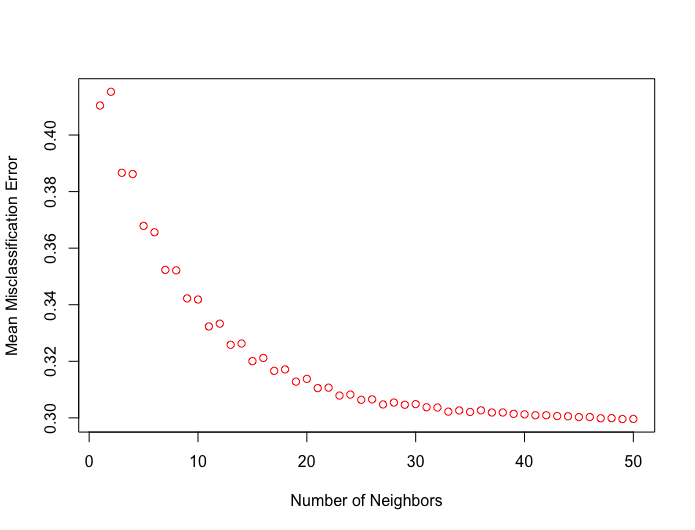
\includegraphics[width = \textwidth]{Rplot02.png}
        \end{center}
      \end{figure}
      \textbf{Code:}
      \begin{center}
      \lstinputlisting[basicstyle = \footnotesize]{r4.txt}
      \end{center}
      I think we might need to use a different evaluation method or more likely the data are too homogenous and finding a model to predict Kredit with these parameters is not very possible.
  \end{enumerate}
\end{exercise}
\vspace{.5in}




\begin{exercise}{2.} Now take the same data as before, but run a linear discriminant analysis using the function lda().\\
  \begin{enumerate}
    \item[a.] Run the analysis and classify all of the data using a rule built by all of the data (i.e. the naive confusion matrix). Does the classification seem
    to work?\\
    \solution Running the linear discriminant analysis using lda(), we get another issue similar to the knn model. It seems as though both models result in applying the a single classification to almost all of 
    the data. I imagine what is causing this is that both of the data groups are lying right on top of each other inside the ellipsoid which spans the data.(I ran the analysis including the variables that we removed in the beginning and still had the same problem). \\
    \textbf{Code:}
      \begin{center}
      \lstinputlisting[basicstyle = \footnotesize]{r5.txt}
      \end{center}
    \vspace{.15in}

    \item[b.] lda() has an argument that performs cross-validation. Use it to get a cross validated confusion matrix. How well do you think the classification
    is working?\\
    \solution Running the cross validated lda we get the the same confusion matrix, because the model in both cases is just assigning the same class to every observation. The data are most definitely not linearly separable
    so it seems its assigning all the observations to the class with the greater proportions.\\
    \textbf{Code:}
      \begin{center}
      \lstinputlisting[basicstyle = \footnotesize]{r6.txt}
      \end{center}
    \vspace{.15in}

    \item[c.] When do you expect linear discriminant analysis to work especially well?\\
    \solution We expect linear discriminant analysis to work best when the data are linearly separable . To some extent we can allow the data to overlap and 
    LDA will provide a suitable mean boundary that can be tuned by priors, as we saw in the examples during class. With the Kredit data the two classes are almost entirely overlapping. 
  \end{enumerate} 
\end{exercise}


\begin{exercise}{3} In problem two, we have the option of setting prior probabilities for each group. The default is to use the actual size of the groups in the data (70
  percent credit-worthy), but you can modify the priors. Run an lda analysis with the prior belief that 40 percent of the population should be credit-
  worthy and 60 percent not. You can just use a testing/training approach for this problem (not cross validation).\\
  \solution Running the LDA with theses priors we get a training accuracy of 0.3238  and a testing accuracy 0.345. When the data are completly indeparble our classifyer before was able to do relatively well 
  by taking advantage of the proportional priors in our data(assigning all observations to largest proportional class size). We cannot assume that credit worthy people make up 70 percent of the population and similarly with non-credit worthy people. In reality our prior models 
  were likely at best randomly assigning credit worthiness. It feels like the only reason we have an accuracy lower than 50\% is because our priors and the proportion of classes in our data are at odds.\\
  \textbf{Code:}
  \begin{center}
  \lstinputlisting[basicstyle = \footnotesize]{r7.txt}
  \end{center}
\end{exercise}
\vspace{.5in}


\begin{exercise}{4} Now repeat problem two, but using quadratic discriminant analysis:\\
  \begin{enumerate}
    \item[a.] Run the analysis and classify all of the data using a rule built by all of the data (i.e. the naive confusion matrix). Does the classification seem
    to work?\\
    \solution Running the analysis we get better spread of classification. The confusion matrix shows that the model predicted 0 for 145 of the 
    observations which in general feels more productive than classifying every observation as a single class even though we achieved slightly lower accuracy at 0.693. I'm surprised that QDA was actually able to achieve this 
    as it seems that, looking at the pair plot the data does not seem to be quadratically separable. \\
    \textbf{Code:}
    \begin{center}
    \lstinputlisting[basicstyle = \footnotesize]{r8.txt}
    \end{center}
    \vspace{.15in}


    \item[b.] qda() has an argument that performs crossvalidation. Use it to get a crossvalidated confusion matrix. How well do you think the
    classification is working?\\
    \solution Generating the cross validated confusion matrix we get an accuracy of 0.639, which seems more representative of a method that is actually predicting some of 
    the observations to be 0.
    \textbf{Code:}
    \begin{center}
    \lstinputlisting[basicstyle = \footnotesize]{r9.txt}
    \end{center}
    \vspace{.15in}

    \item[c.] When do you expect quadratic discriminant analysis to work especially well?\\
    \solution  We expect quadratic discriminant analysis to work best when the data are quadratically separable (what does one of these decision boundaries look like in 3d and hyperspace? Are they degenerate like a cylinder or 
    non-degenerate like an ellipsoid?).
    \vspace{.15in}



    \item[d.] Of the models (Mahalanobis, k-nearest neighbor, linear discriminant, and quadratic discriminant), which are most likely to overfit the data?
Which are most likely to underfit the data?\\
\solution What you are describing is the bias-variance tradeoff that each model has. KNN has the property that it can underfit with large values of k and overfit with small values of K (like a tree, it has options). 
Generally LDA and QDA are methods that underfit the data. I can imagine the Mahalanobis classifier making curved decision boundaries similar to QDA so it also likely underfits data. 

  \end{enumerate}
  
\end{exercise}
\vspace{.15in}

\begin{exercise}{5} Which of the analyses you did in this assignment did you prefer? Did one seem to work better with the variables you selected?\\
  \solution I preferred KNN. I like how we can tune it like decision trees to over and underfit the data. It seems like boosting them leads to a form of weighted KNN. I don't think bagging them 
  will lead to substantially better results since bootstrapping the data will likely give similar decision boundaries. I'm not sure if I did a bad job preparing the data, from the pair plot and MANOVA 
  it seems like they were right on top of each other which makes discriminant analysis difficult. The QDA model seemed to actually acknowledge the other class in the data so I wonder if there is some sort of 
  transformation in the predictors that really separates the data. 
\end{exercise}



\end{document}


















